\label{multiProt}
The focus in this section is on interactions occurring between multiple FAK molecules, which are obtained from setup 4. At this point we want to remind the reader that the used protein structure lacks the FAT domain, which is in full length FAK connected to the kinase via a linker region. This might have a significant effect on clustering processes.
\subsection{Dimerization of FAK}
\label{mult:dimers}
First, we want to investigate interactions between two FAK molecules. For this purpose we filtered the dataset for interactions, in which both partners have exactly one neighbour. It turns out that FERM-kinase dimers occur the most followed by FERM-FERM dimers. Because the latter have been experimentally investigated by \textcite{fakdimers} a short comparison between the obtained results and the experimental findings is given. For this purpose we chose the dimer with the longest lasting time as a representative example.\\ % TODO: add the plot here? 
\\
The contact map of the interaction surface is shown in \autoref{mult:fermfermcontact}. From this the importance of residue \acid{W}{266} can be confirmed (orange region). Beside this also the residues \acid{Y}{282} to \acid{K}{286} (green region), \acid{T}{291} to \acid{A}{394} (red region) and \acid{G}{322} to \acid{L}{327} (violet region) appear as important actors at the interaction surface since they interact with \acid{W}{266} and among each other. However, the RMSF value of these contacts is larger than for the contacts involving \acid{W}{266}.\\
At this point it has to be said that other FERM-FERM dimers in the simulation show also contacts between F1 and F3. Since they are not visible in other samples (e.g. the chosen one), they are not presented here.\\
% TODO: difference to paper?, not really, because they have no membrane
FERM-FERM dimerization affects the FERM kinase interface of the involved proteins. In comparison to FAK-MEM almost all distances of the interacting residues gets closer for both protein instances (about $0.2\,\si{\nano\metre}$). A reason for this could be that the connection of the FERM domains require an uplift of F3 since the interaction interface points towards the membrane in FAK-MEM. Because the FERM domain is anchored on the membrane via the basic patch, this would push the kinase partly into the membrane. Therefore a force is acting on the kinase, which could be the reason of the closure. % TODO: cite Daniel?
%
%
%
\begin{figure}
	\centering
	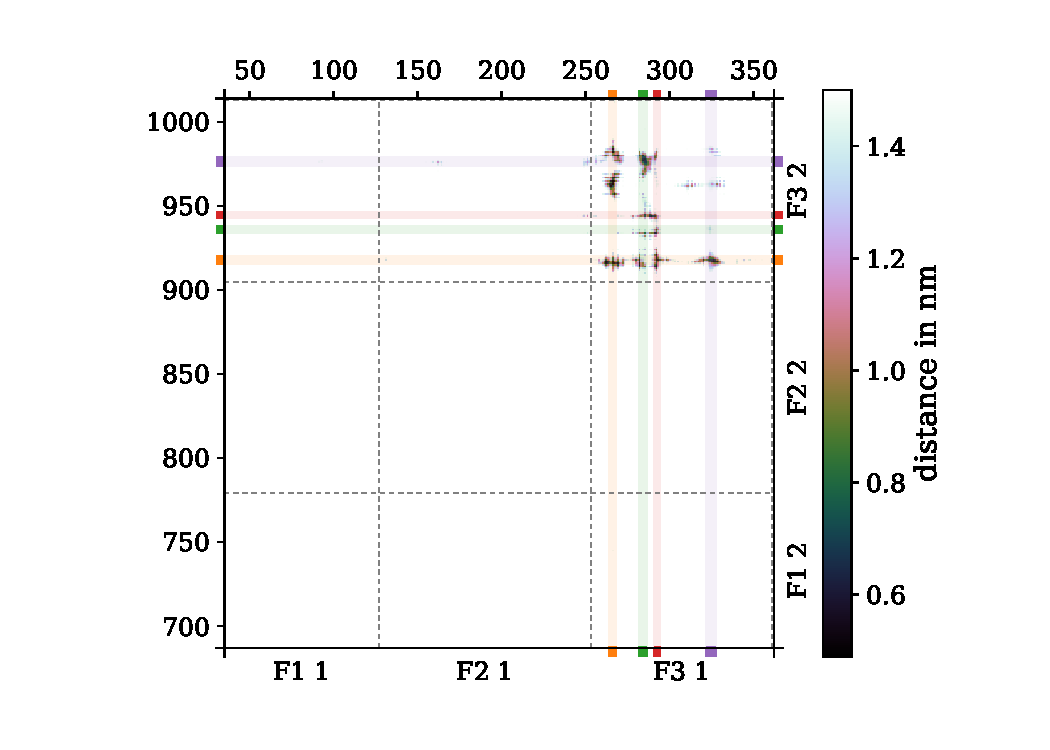
\includegraphics[width=.8\textwidth]{figures/results/fermferminterface}
	\nicecaption{Contactmap of FERM-FERM dimers}{The contact map shows the interaction site. The most important residues are highlighted.}
	\label{mult:fermfermcontact}
\end{figure}
%
%
%
\subsection{FAK clusters}
\label{mult:oligs}
The characterisation of the emerged FAK clusters is very difficult as they differ a lot in size and shape. The largest cluster observed in setup 4 had a size of 21 proteins, while there are other proteins, which did not join any cluster at all. Present shapes of the clusters include long chains as well as ring like conformations or just agglomerations (see \autoref{tobeadded}). \\
\\
First of all we focus on the occurring neighbouring types, which were introduced in \autoref{methods:contactana}. In \autoref{mult:inttype_vs_t} the time evolution of the average number of encounters of the different interaction types is determined. It shows, that FERM-kinase interactions (type 3) occur the most, while type 1, 2, 4 and 5 occur equally often. Type 6 and type 7 are interactions, in which all four domains are involved. They occur less often, especially type 7, which is the asymmetric one.\\
We also analysed the altering of neighbour types, which is presented in \autoref{mult:inttype_markov}. This indicates that the first contact of two FAK molecules appear at the end of their long axis. Some of these in line neighbours alter than to type 4 and 5, but also backwards. Also type 6 neighbours are only formed out of already interacting proteins.\\
Lastly the mean number of neighbours is considered. It turns out, that there is a fast rising in the beginning and a flattening after $6\,\si{\nano\second}$. The average over the five copies is at the end of the simulation $1.86$ neighbours.\\
From these observations one could draw the conclusion, that the preferred arrangement of FAK molecules are chains along their long axis. The FAK molecules inside the chain interact either as type 3 (FK chains) neighbours or as type 1 and type 2 neighbours (FFKK chains). Of course also combinations of these two are possible.
%
%
%
\begin{figure}
	\subcaptionbox{\label{mult:inttype_vs_t}}[0.49\textwidth]{
		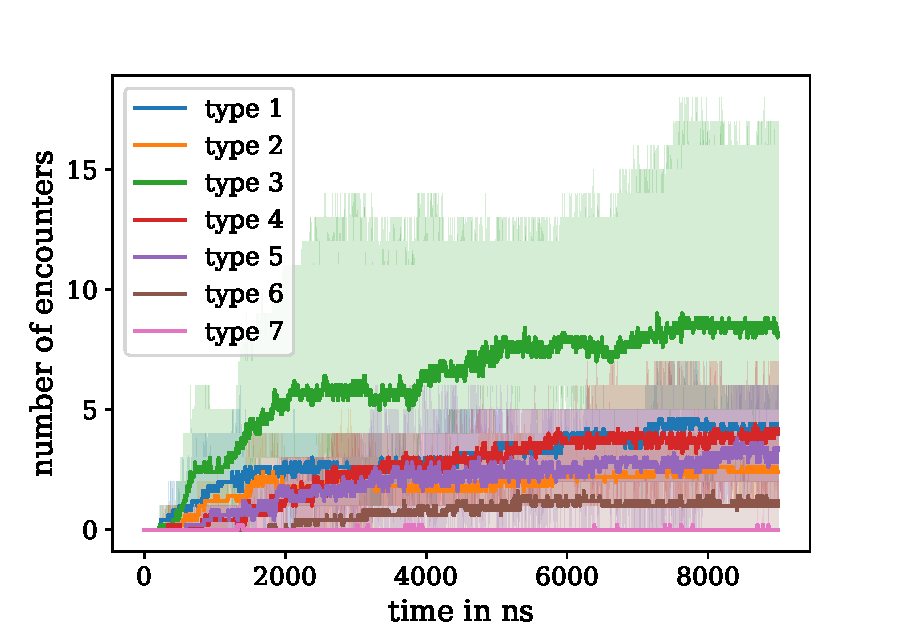
\includegraphics[height=5cm]{figures/results/multiple_typevstime}
	}\hfill%
	\subcaptionbox{\label{mult:inttype_markov}}[0.49\textwidth]{
		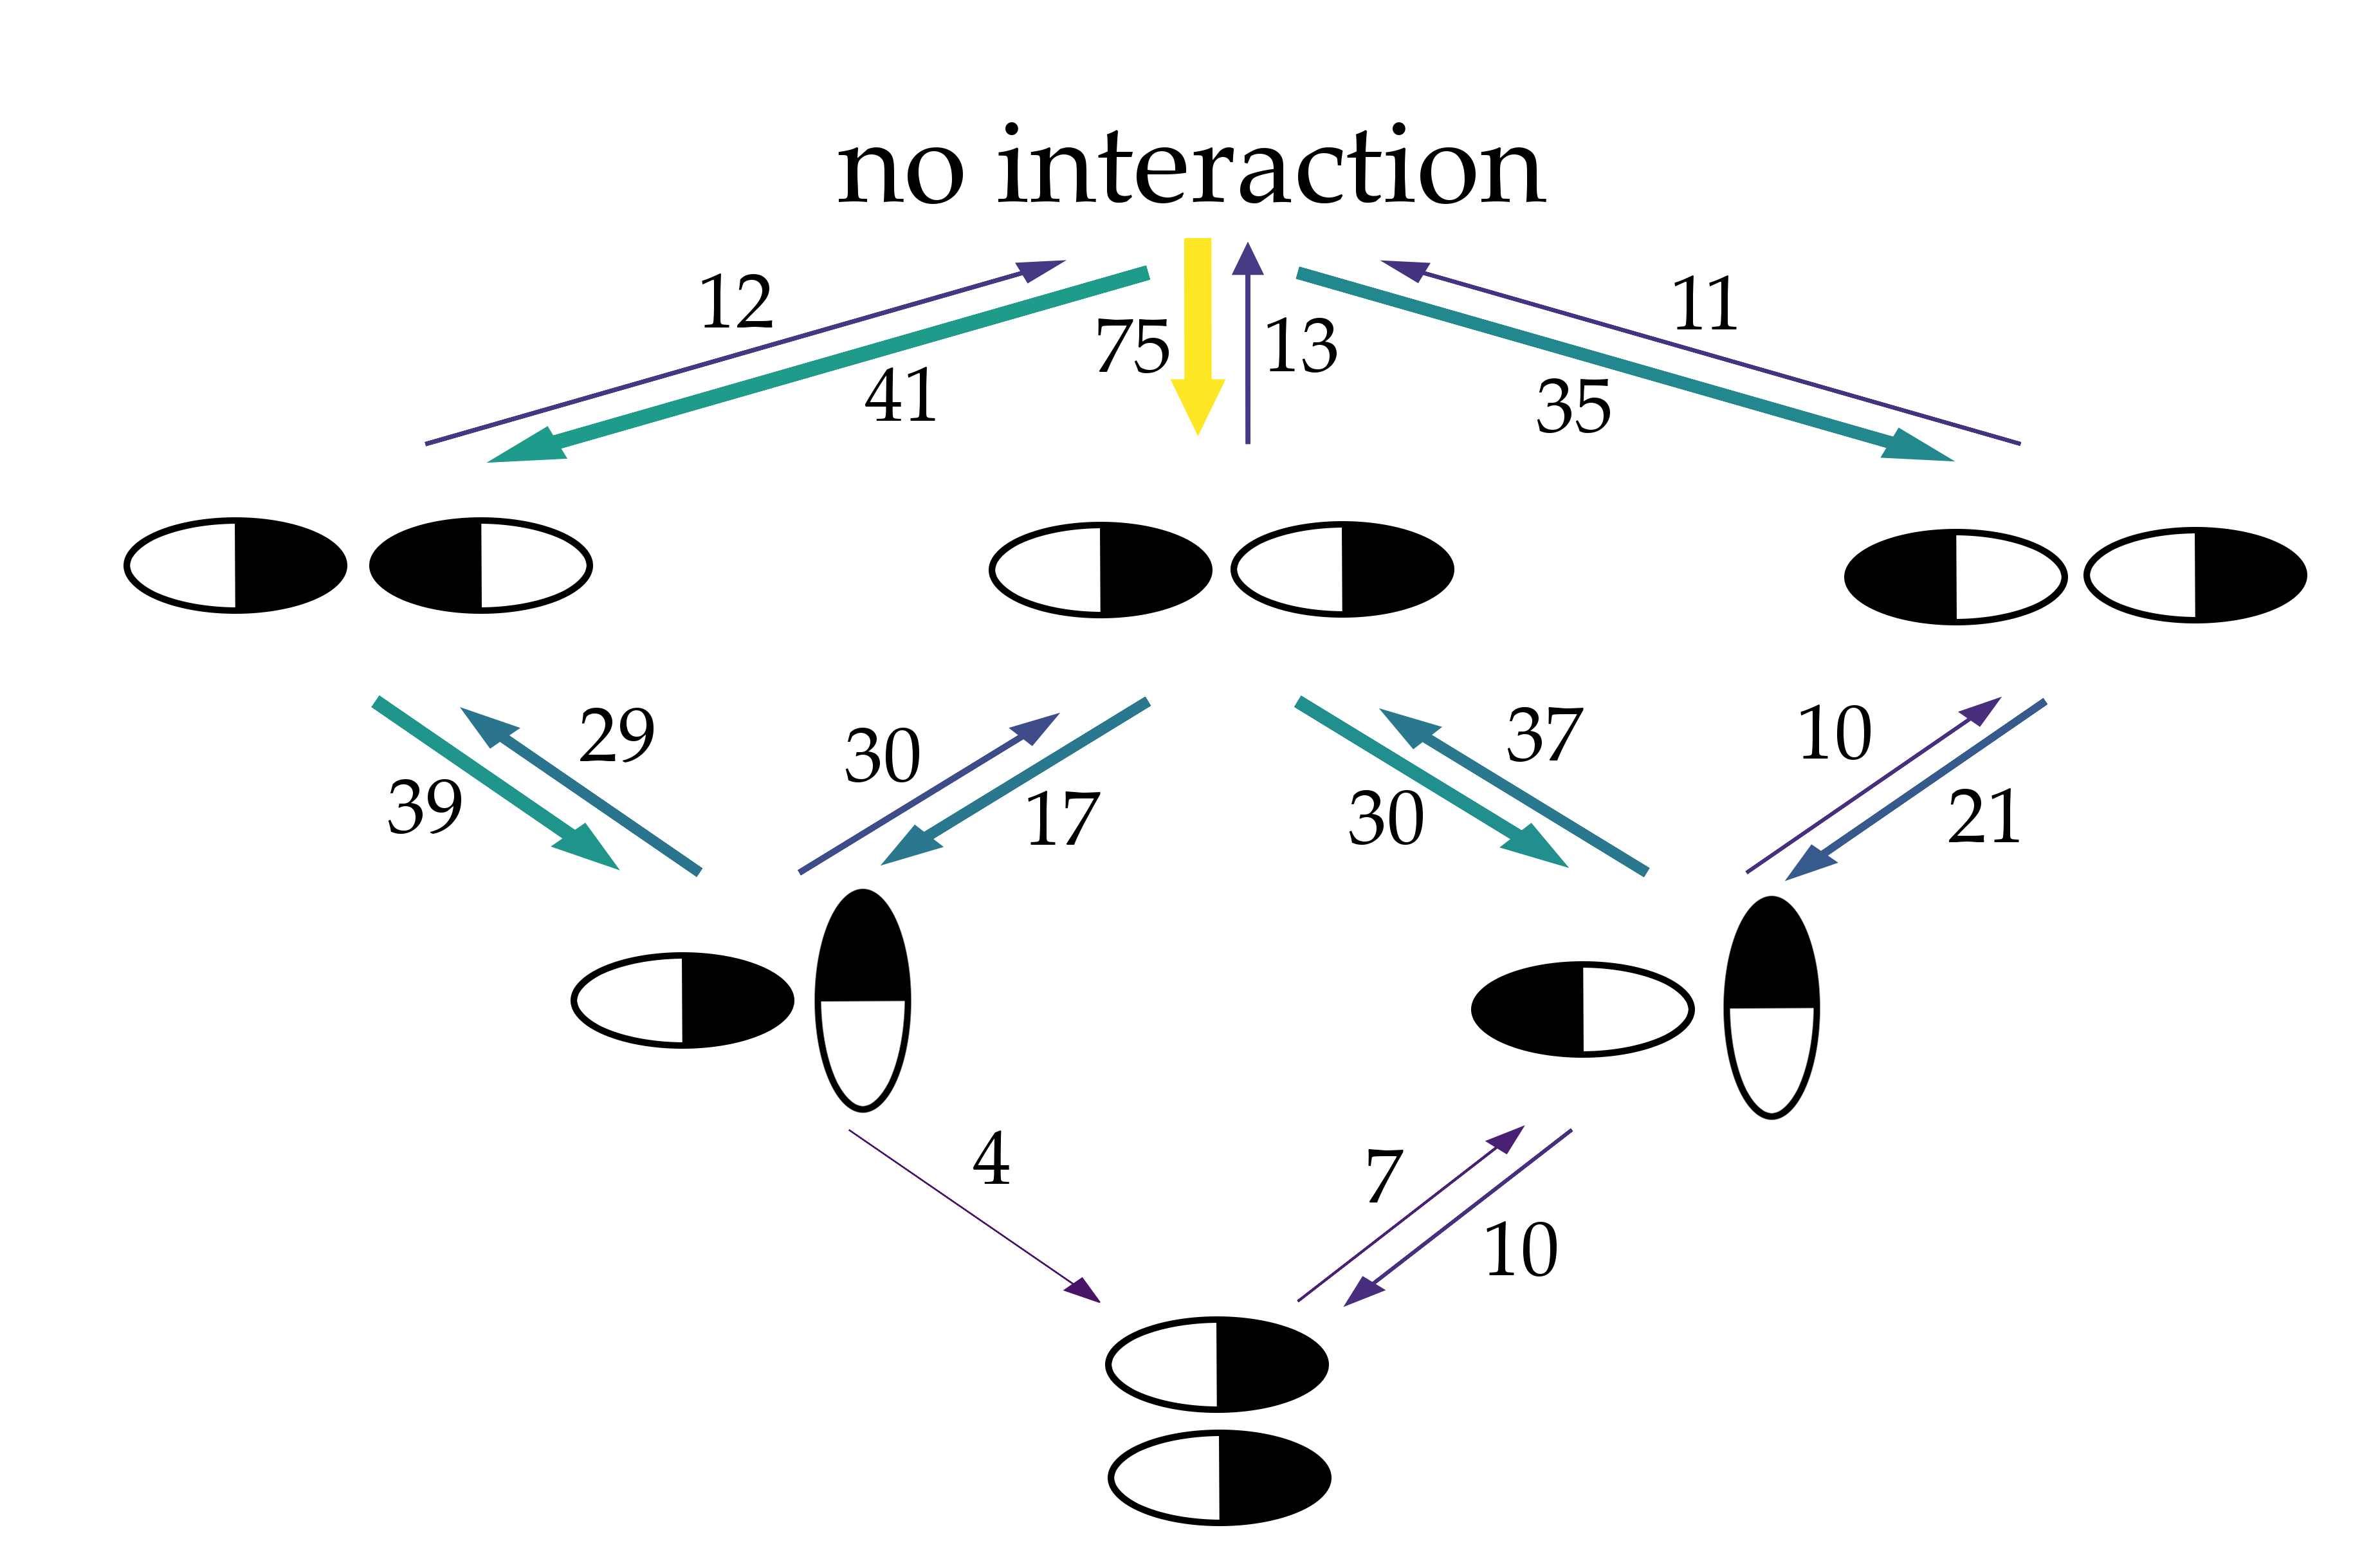
\includegraphics[height=5cm]{figures/results/markov}
	}%
	\nicecaption{Evolution of neighbouring types}{(\subref{mult:inttype_vs_t}): Mean number of encounters over the five copies for the different neighbouring types. The filled area shows the range from minimum to maximum. (\subref{mult:inttype_markov}): Transition diagram of the neighbouring types. Width and colour of the arrows correspond to the total number of observed transitions, which is also given beside the arrows.}
\end{figure}
%
%
%
\subsection{Activation due to clustering}
Lastly, the impacts of clustering on FAK activation are addressed. Activation means here the dissociation of the FERM domain from the kinase, therefore we analysed our data with respect to the contact area (CA) of the FERM-kinase interface.\\
Unfortunately in no FAK molecule did a full dissociation take place at any time. Because only a small number of FAK molecules were in the system and because the clustering process is not finished at the end of the simulations, this does not mean, that activation due to clustering would not be possible at all. In the hope of seeing trends regarding to activation a more detailed analysation of the CA for the different proteins was performed.\\
\\
At first glance CA seems to be independent of the number of neighbours (\autoref{mult:nng_ca}), the interaction type and the clustersize.\\
Motivated from \autoref{mult:oligs} we focus on FAK molecules inside chains in the following. A FAK molecule can be seen as a chain member, if it has exactly two neighbours and if these neighbours are not neighbours of one another. For FK chains only type 3 interactions were allowed, for FFKK chains both, type 1 and type 2. We compare the results to FAK-MEM in \autoref{mult:fk_ca} for FK chains and in \autoref{mult:ff_ca} for FFKK chains.\\
\autoref{mult:fk_ca} indicates that an arrangement of FAK molecules to FK chains does not influence the mean value of CA. The distribution gets slightly sharper compared to FAK-MEM, which could imply a stabilisation of the interface. Not even the distributions of $d_\text{F1-N}$ and $d_\text{F2-C}$ differs from those obtained in FAK-MEM.\\
Also an arrangement to FFKK chains affects the value of CA hardly (\autoref{mult:ff_ca}). The distribution gets slightly sharper and shifted to smaller values by $0.6\,\si{\nano\metre}$. However, the distribution of $d_\text{F1-N}$ indicates a trend to larger values in comparison to FAK-MEM, which refers to an more open state of FAK.\\
\\
The filtering leads of course to a smaller sampling of the distributions of $d_\text{F1-N}$, $d_\text{F2-C}$ and CA . E.g. for FFKK chains only 10 different FAK instances were taken into account ($21.7\,\si{\micro\second}$ simulation time in total). However, the obtained changes are visible in almost all of the 10 instances.
%
%
%
%\begin{figure}
%	\centering
%	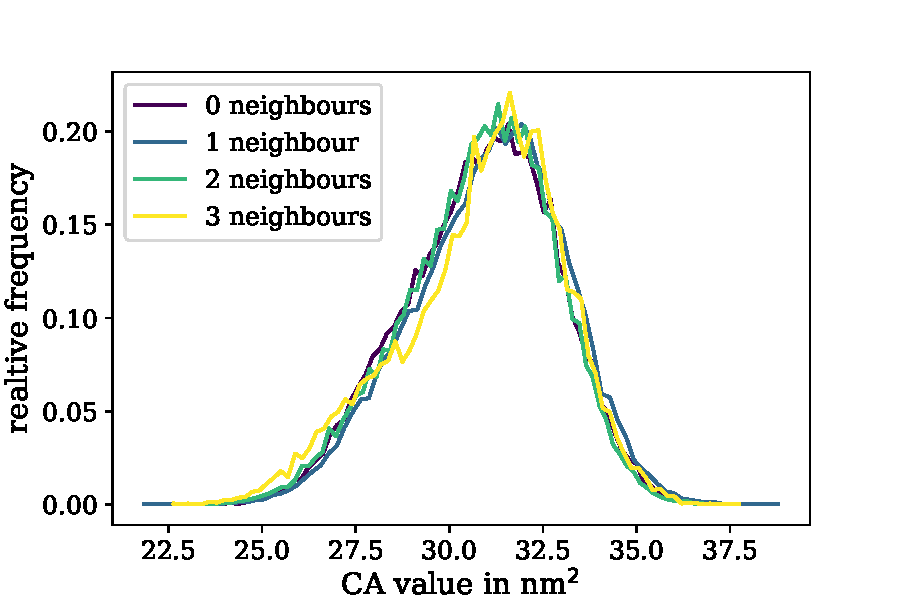
\includegraphics[height=5cm]{figures/results/nng_ca}
%	\nicecaption{CA for different numbers of neighbours}{}
%	\label{mult:nng_ca}
%\end{figure}
%
%
%
%
%
%
\begin{figure}
	\centering
	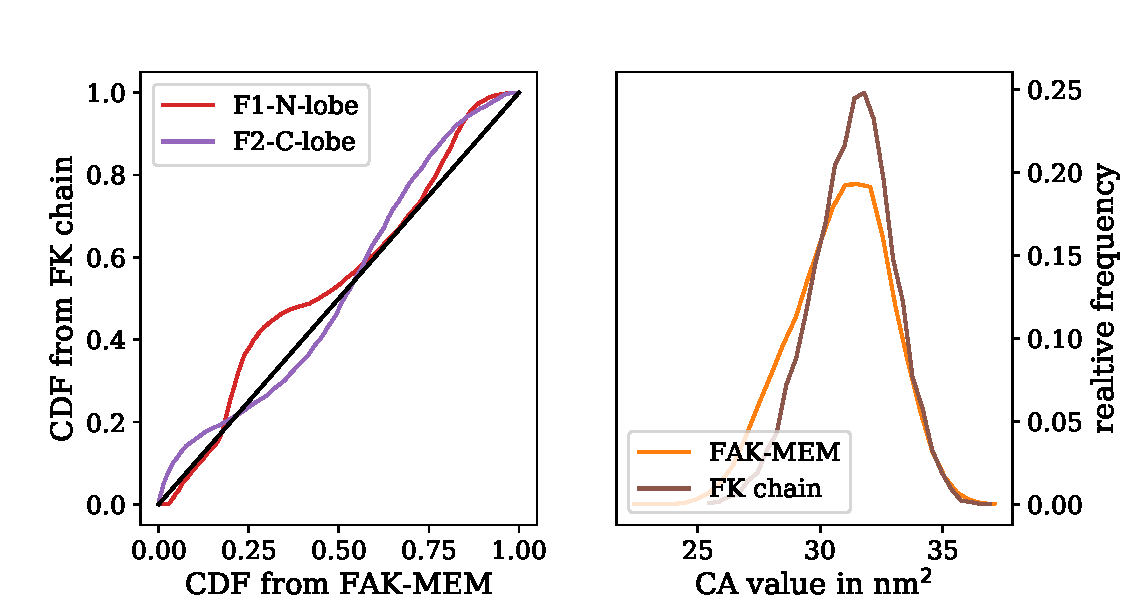
\includegraphics[height=6cm]{figures/results/fk_ca}
	\nicecaption{Domain distances and contact area of FK chains}{(left): Q-Q plot of $d_\text{F1-N}$ and $d_\text{F2-C}$ distributions in comparison to FAK-MEM. The distributions are quit similar. (right): CA value in comparison to FAK-MEM.}
	\label{mult:fk_ca}
\end{figure}
%
%
%
%
%
%
%
\begin{figure}
	\centering
	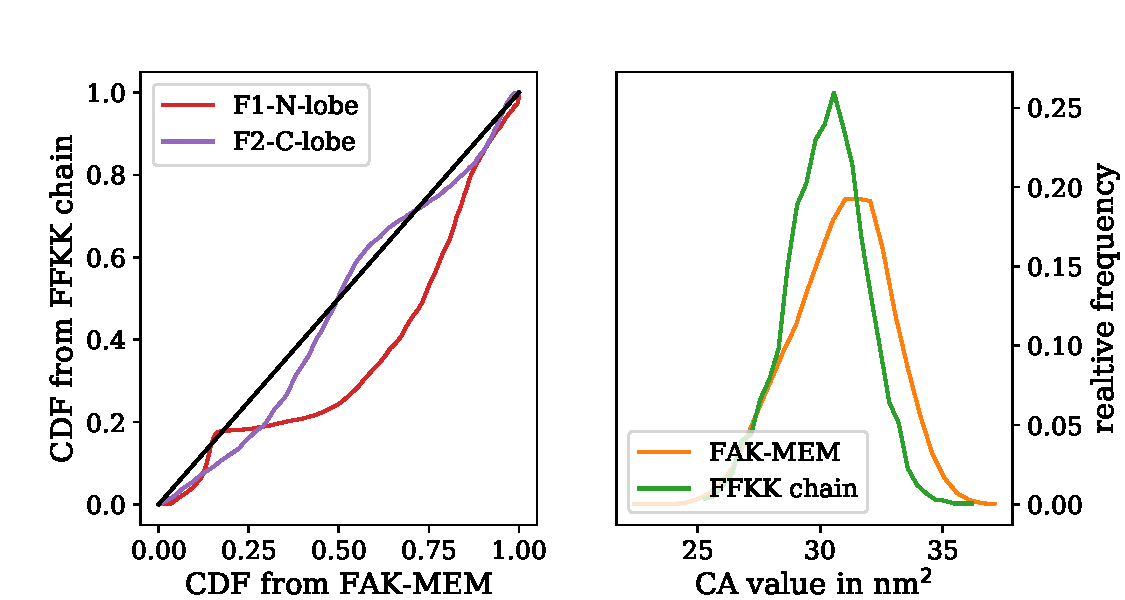
\includegraphics[height=6cm]{figures/results/ff_ca}
	\nicecaption{Domain distances and contact area of FFKK chains}{(left): Q-Q plot of $d_\text{F1-N}$ and $d_\text{F2-C}$ distributions in comparison to FAK-MEM. FFKK chain members tend to larger values of $d_\text{F1-N}$. (right): CA value in comparison to FAK-MEM.}
	\label{mult:ff_ca}
\end{figure}
%
%
%
%
